% ------------------------------------------------------------------------------
% 7.4. DISEÑAR CASO DE USO
% ------------------------------------------------------------------------------
\subsection{7.4. Diseñar Caso de Uso}\label{sec:cap7_disenar_cu}

El diseño de cada caso de uso se expresa mediante diagramas de secuencia, que muestran el orden temporal de los mensajes intercambiados entre el actor y los objetos que realizan el caso de uso \parencite{booch2005uml}. Siguiendo el Proceso Unificado de Desarrollo de Software, cada diagrama de secuencia refina el diagrama de colaboración del análisis (sección~\ref{sec:cap6_analisis_cu}) y conserva sus clases de interfaz (\textit{View}), control (\textit{Controller}) y entidad, incorporando los mensajes de retorno y los fragmentos combinados que representan las alternativas del flujo \parencite{jacobson1999unified}.

A continuación se presenta el diseño de los veintiséis casos de uso del sistema, en el orden de su numeración (CU-01 a CU-26).

\subsubsection{7.4.1. Diseñar CU-01 Registrarse y autenticarse}\label{sec:cap7_disenar_cu01}


\subsubsection{7.4.2. Diseñar CU-02 Enviar postulación a Beca Comedor}\label{sec:cap7_disenar_cu02}


\subsubsection{7.4.3. Diseñar CU-03 Precalificar postulación con Inteligencia Artificial}\label{sec:cap7_disenar_cu03}


\subsubsection{7.4.4. Diseñar CU-04 Consultar estado de postulación}\label{sec:cap7_disenar_cu04}


\subsubsection{7.4.5. Diseñar CU-05 Auditar y adjudicar becas}\label{sec:cap7_disenar_cu05}

La Figura~\ref{fig:secuencia_cu05} presenta el diagrama de secuencia del CU-05.

\begin{figure}[H]
\caption{Diagrama de secuencia del CU-05 Auditar y adjudicar becas}
\label{fig:secuencia_cu05}
\centering
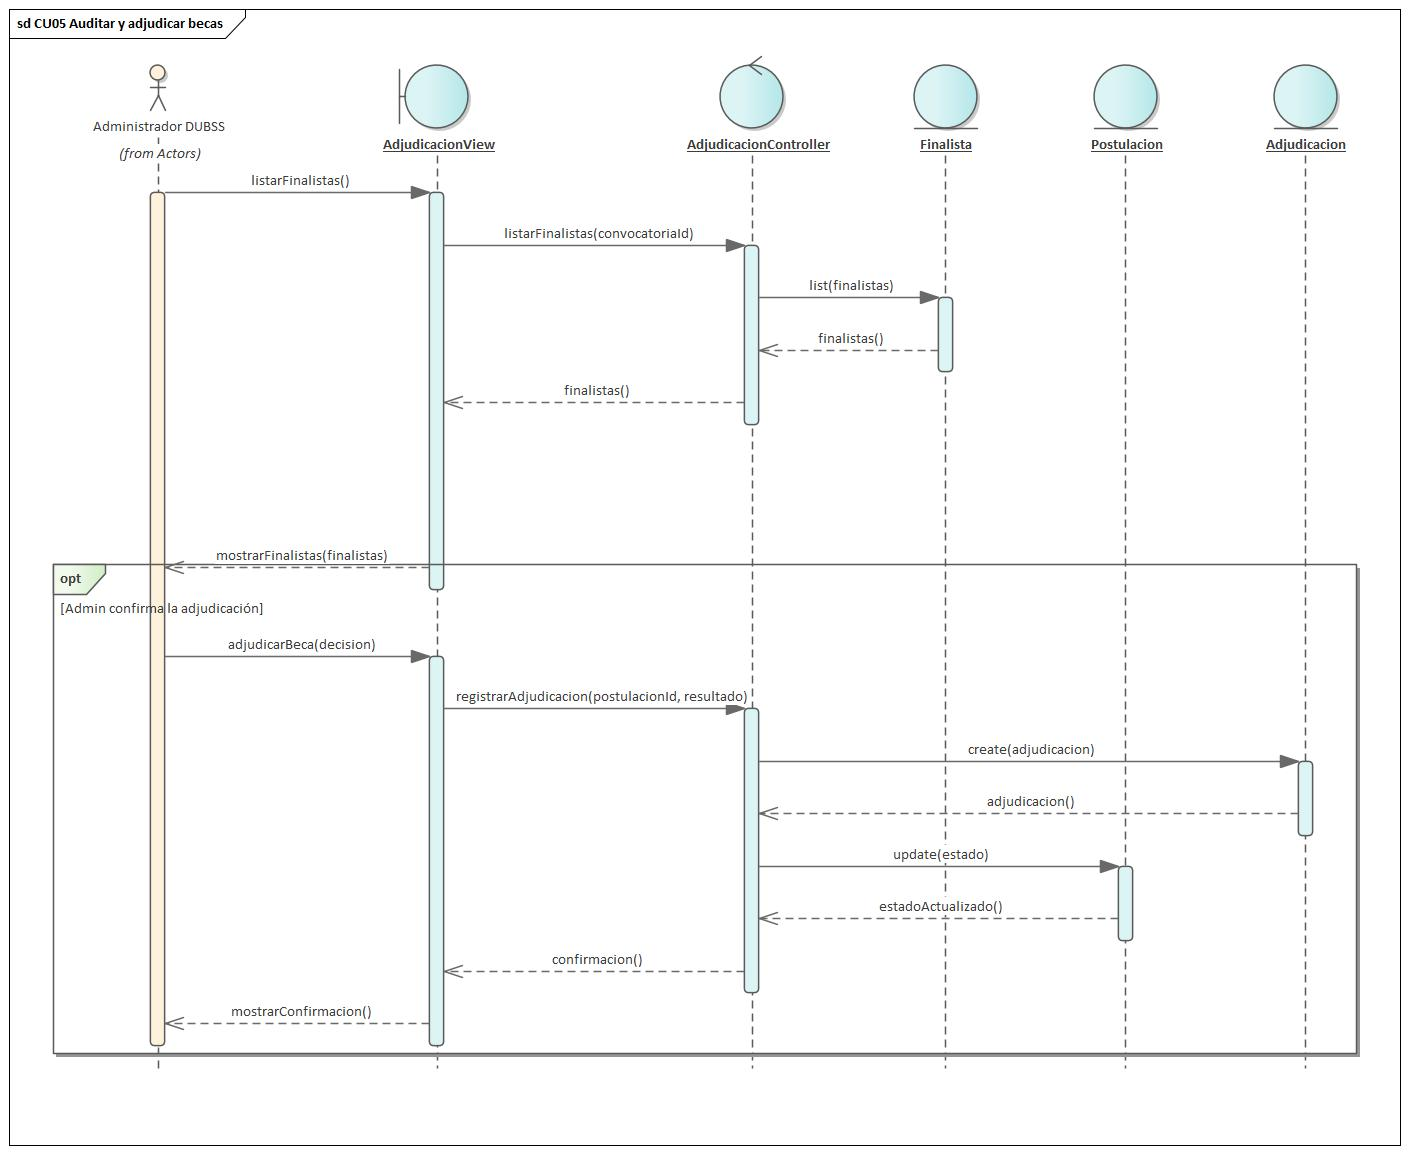
\includegraphics[width=\textwidth,height=0.75\textheight,keepaspectratio]{images/092_Secuencia_CU05_Auditar_Adjudicar_Becas.jpg}

\smallskip
\noindent\raggedright\textit{Nota.} Elaboración propia.
\end{figure}


\subsubsection{7.4.6. Diseñar CU-06 Visualizar lista priorizada de postulantes}\label{sec:cap7_disenar_cu06}

La Figura~\ref{fig:secuencia_cu06} presenta el diagrama de secuencia del CU-06.

\begin{figure}[H]
\caption{Diagrama de secuencia del CU-06 Visualizar lista priorizada de postulantes}
\label{fig:secuencia_cu06}
\centering
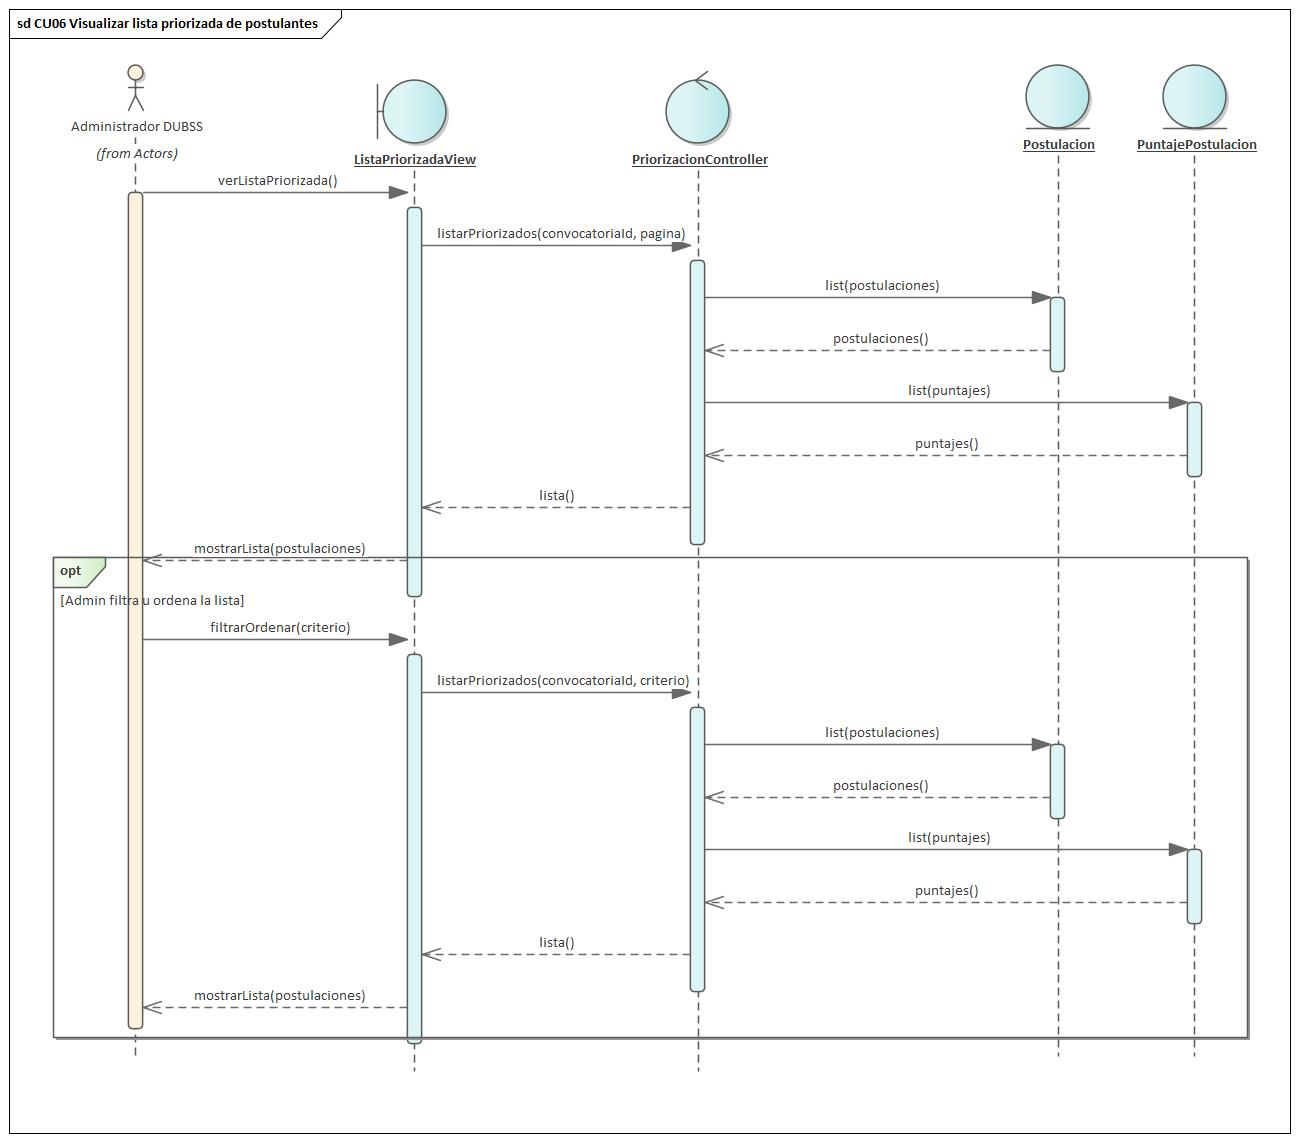
\includegraphics[width=\textwidth,height=0.75\textheight,keepaspectratio]{images/093_Secuencia_CU06_Visualizar_Lista_Priorizada_Postulantes.jpg}

\smallskip
\noindent\raggedright\textit{Nota.} Elaboración propia.
\end{figure}


\subsubsection{7.4.7. Diseñar CU-07 Auditar expediente finalista}\label{sec:cap7_disenar_cu07}

La Figura~\ref{fig:secuencia_cu07} presenta el diagrama de secuencia del CU-07.

\begin{figure}[H]
\caption{Diagrama de secuencia del CU-07 Auditar expediente finalista}
\label{fig:secuencia_cu07}
\centering
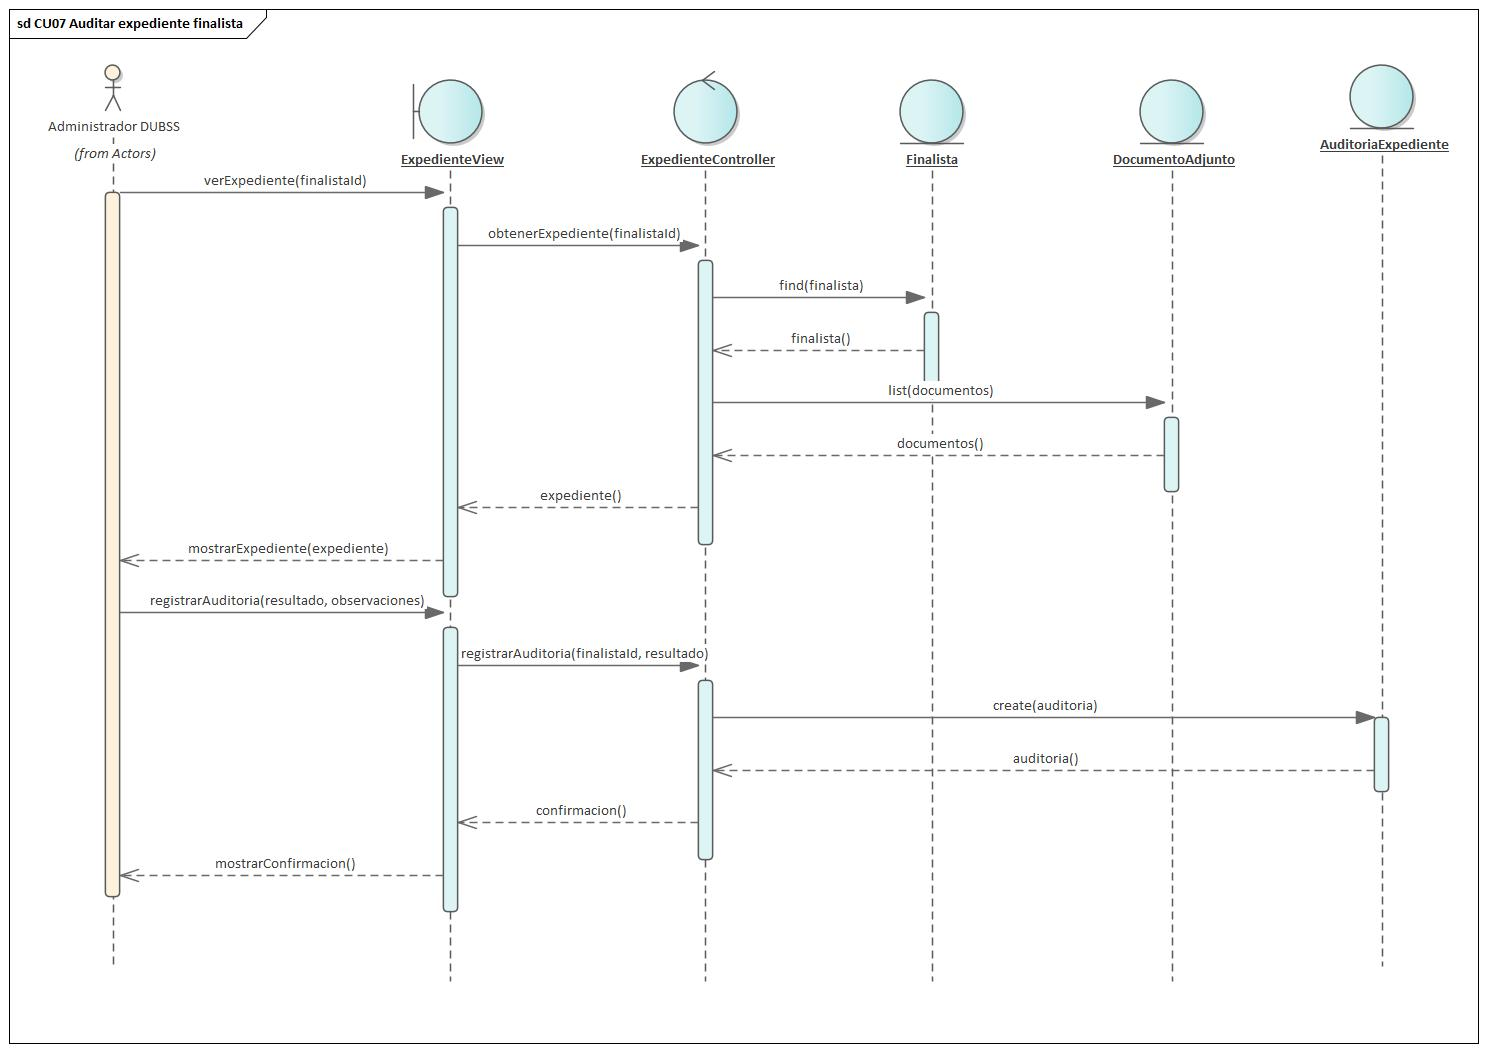
\includegraphics[width=\textwidth,height=0.75\textheight,keepaspectratio]{images/094_Secuencia_CU07_Auditar_Expediente_Finalista.jpg}

\smallskip
\noindent\raggedright\textit{Nota.} Elaboración propia.
\end{figure}


\subsubsection{7.4.8. Diseñar CU-08 Generar acta de adjudicación}\label{sec:cap7_disenar_cu08}

La Figura~\ref{fig:secuencia_cu08} presenta el diagrama de secuencia del CU-08.

\begin{figure}[H]
\caption{Diagrama de secuencia del CU-08 Generar acta de adjudicación}
\label{fig:secuencia_cu08}
\centering
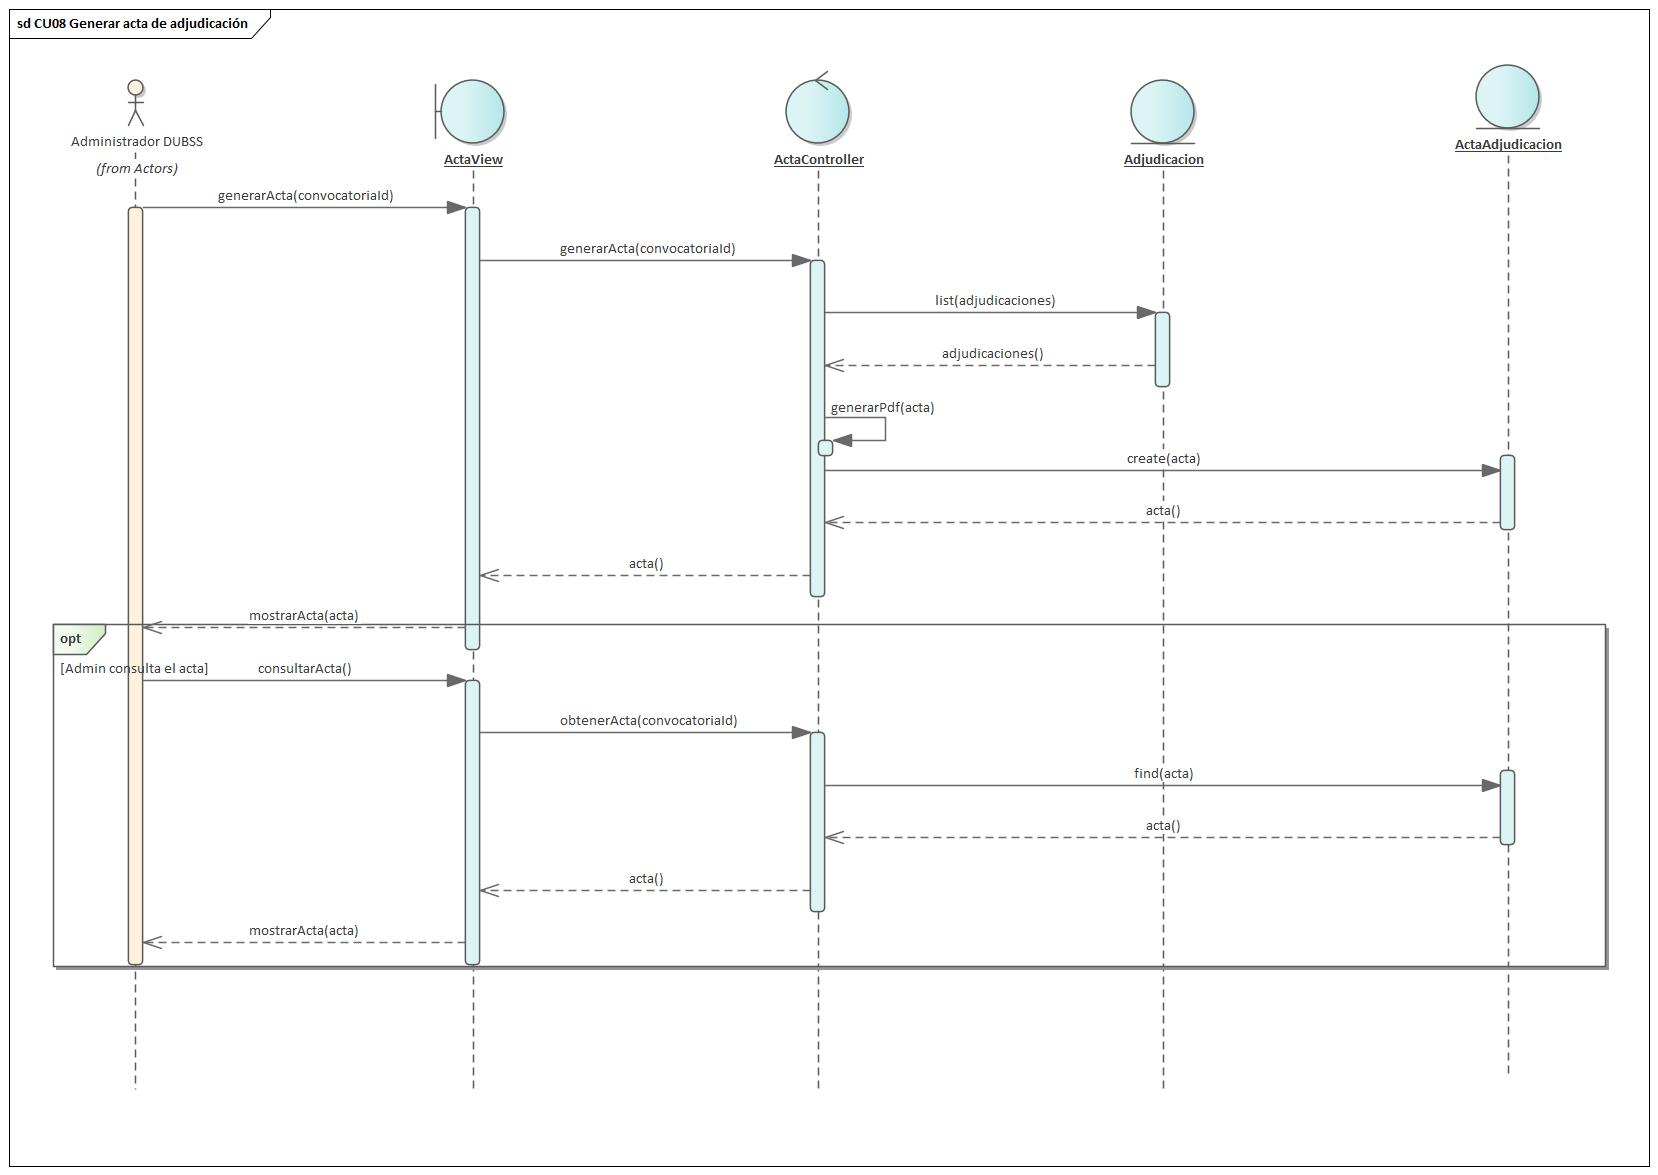
\includegraphics[width=\textwidth,height=0.75\textheight,keepaspectratio]{images/095_Secuencia_CU08_Generar_Acta_Adjudicacion.jpg}

\smallskip
\noindent\raggedright\textit{Nota.} Elaboración propia.
\end{figure}


\subsubsection{7.4.9. Diseñar CU-09 Generar planilla de asistencia}\label{sec:cap7_disenar_cu09}

La Figura~\ref{fig:secuencia_cu09} presenta el diagrama de secuencia del CU-09.

\begin{figure}[H]
\caption{Diagrama de secuencia del CU-09 Generar planilla de asistencia}
\label{fig:secuencia_cu09}
\centering
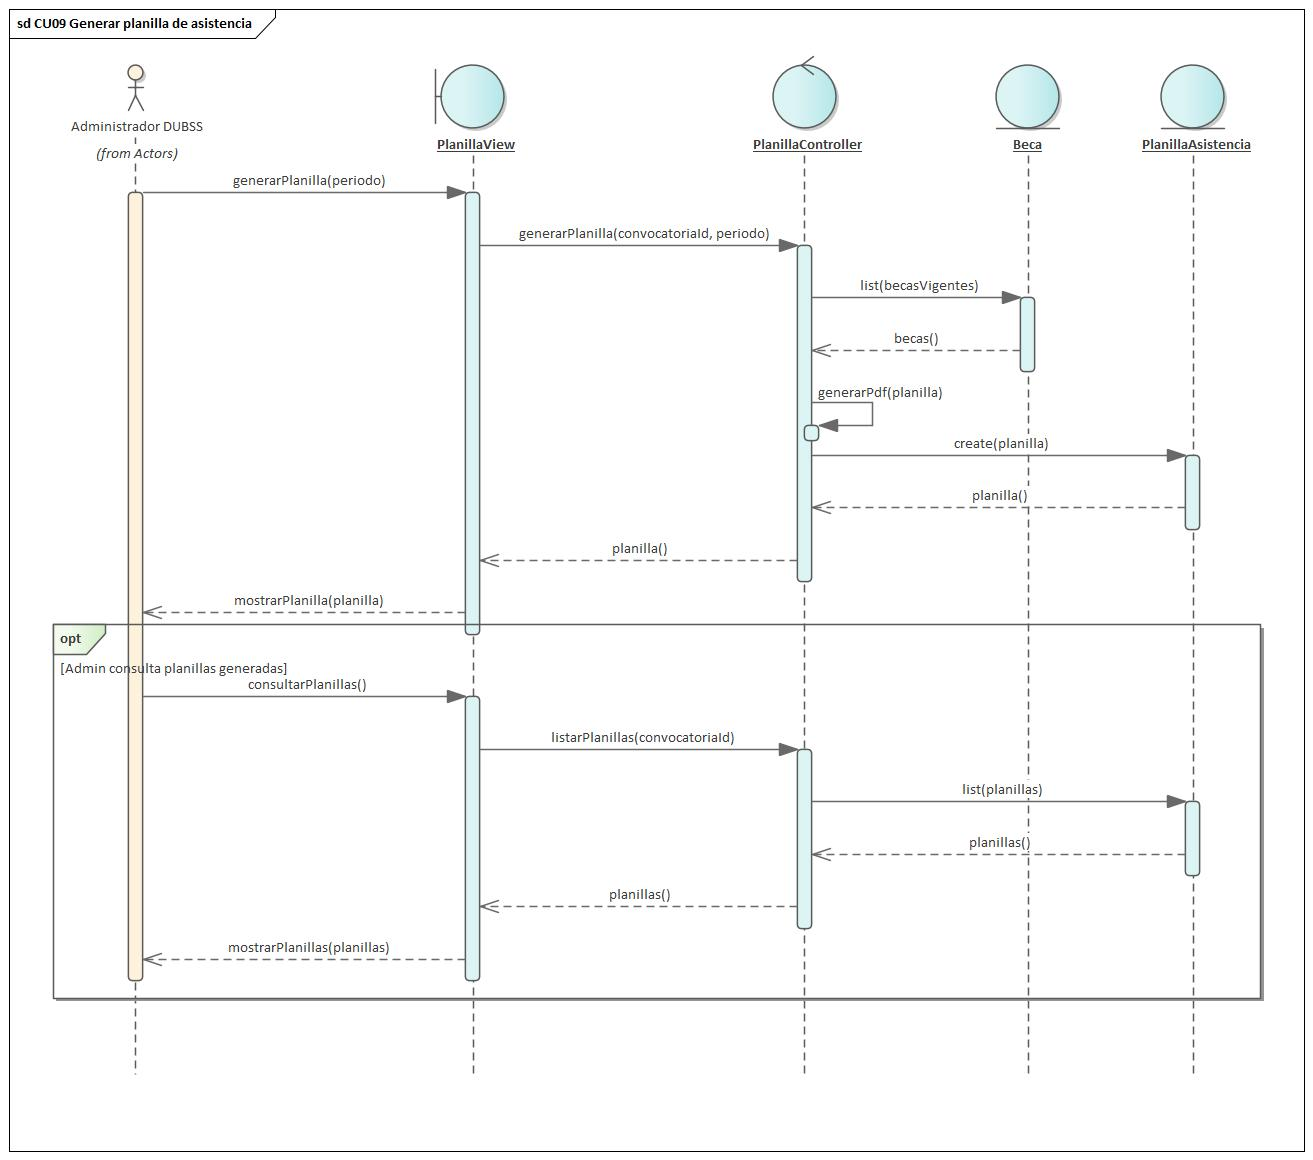
\includegraphics[width=\textwidth,height=0.75\textheight,keepaspectratio]{images/096_Secuencia_CU09_Generar_Planilla_Asistencia.jpg}

\smallskip
\noindent\raggedright\textit{Nota.} Elaboración propia.
\end{figure}


\subsubsection{7.4.10. Diseñar CU-10 Registrar asistencia digital}\label{sec:cap7_disenar_cu10}

La Figura~\ref{fig:secuencia_cu10} presenta el diagrama de secuencia del CU-10.

\begin{figure}[H]
\caption{Diagrama de secuencia del CU-10 Registrar asistencia digital}
\label{fig:secuencia_cu10}
\centering
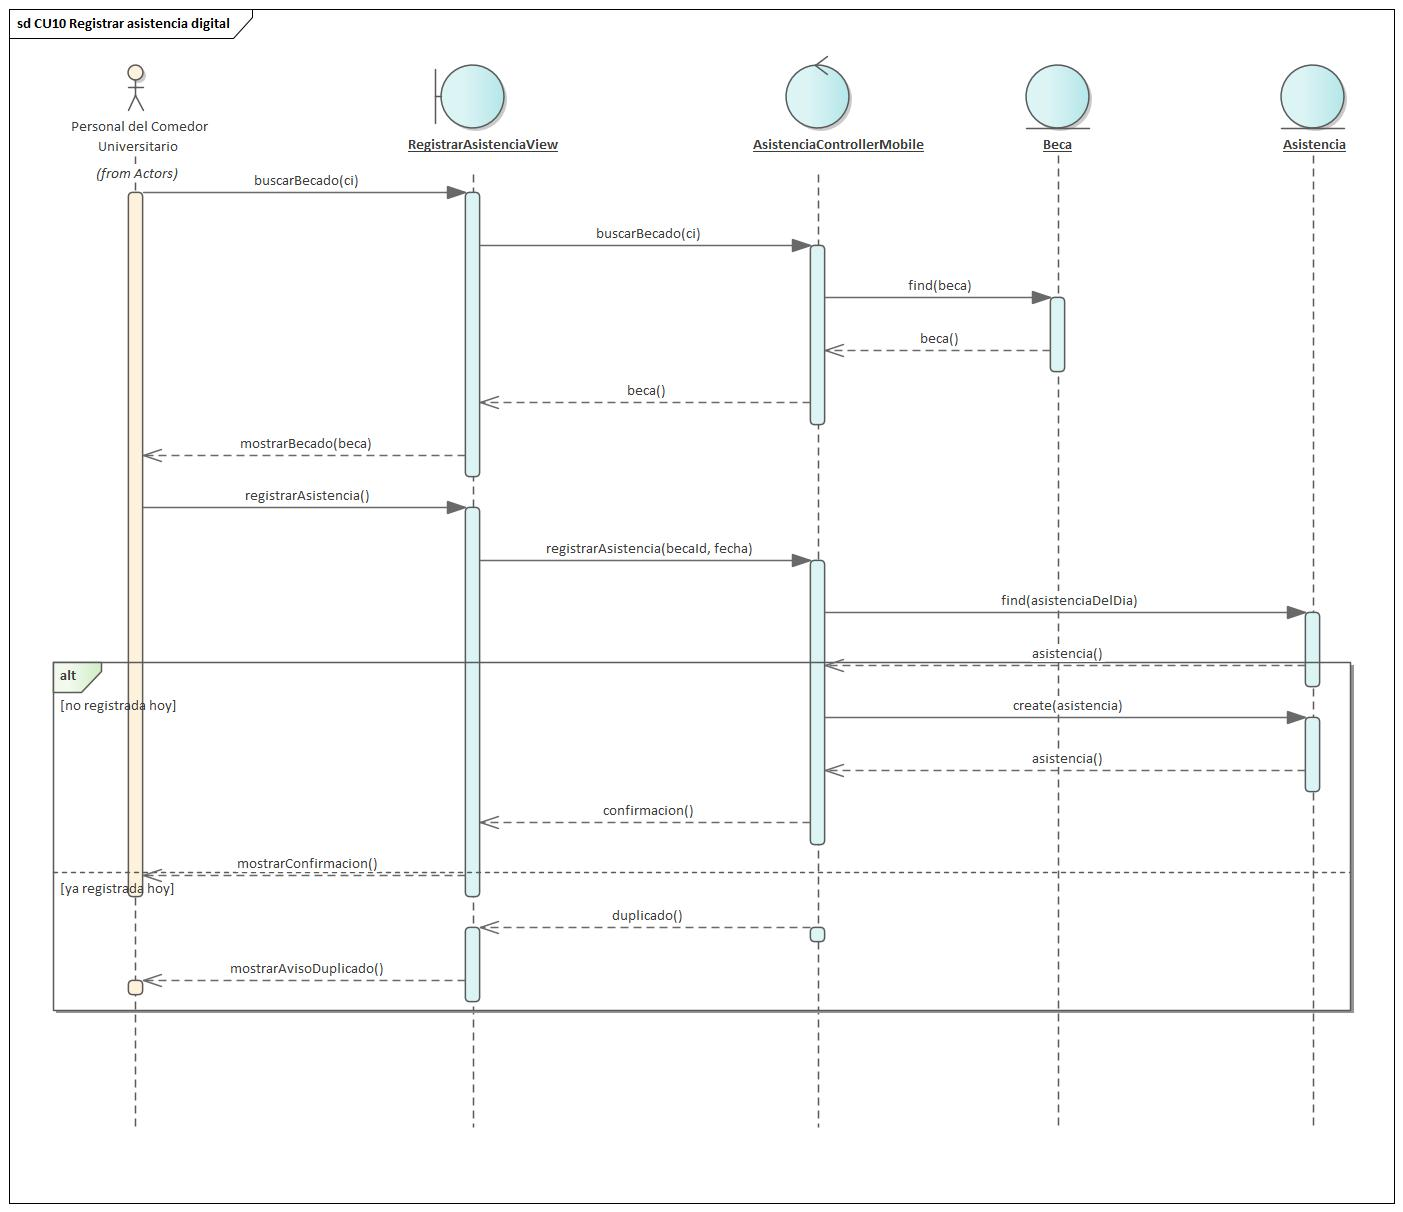
\includegraphics[width=\textwidth,height=0.75\textheight,keepaspectratio]{images/097_Secuencia_CU10_Registrar_Asistencia_Digital.jpg}

\smallskip
\noindent\raggedright\textit{Nota.} Elaboración propia.
\end{figure}


\subsubsection{7.4.11. Diseñar CU-11 Cotejar registro contra respaldo físico}\label{sec:cap7_disenar_cu11}

La Figura~\ref{fig:secuencia_cu11} presenta el diagrama de secuencia del CU-11.

\begin{figure}[H]
\caption{Diagrama de secuencia del CU-11 Cotejar registro contra respaldo físico}
\label{fig:secuencia_cu11}
\centering
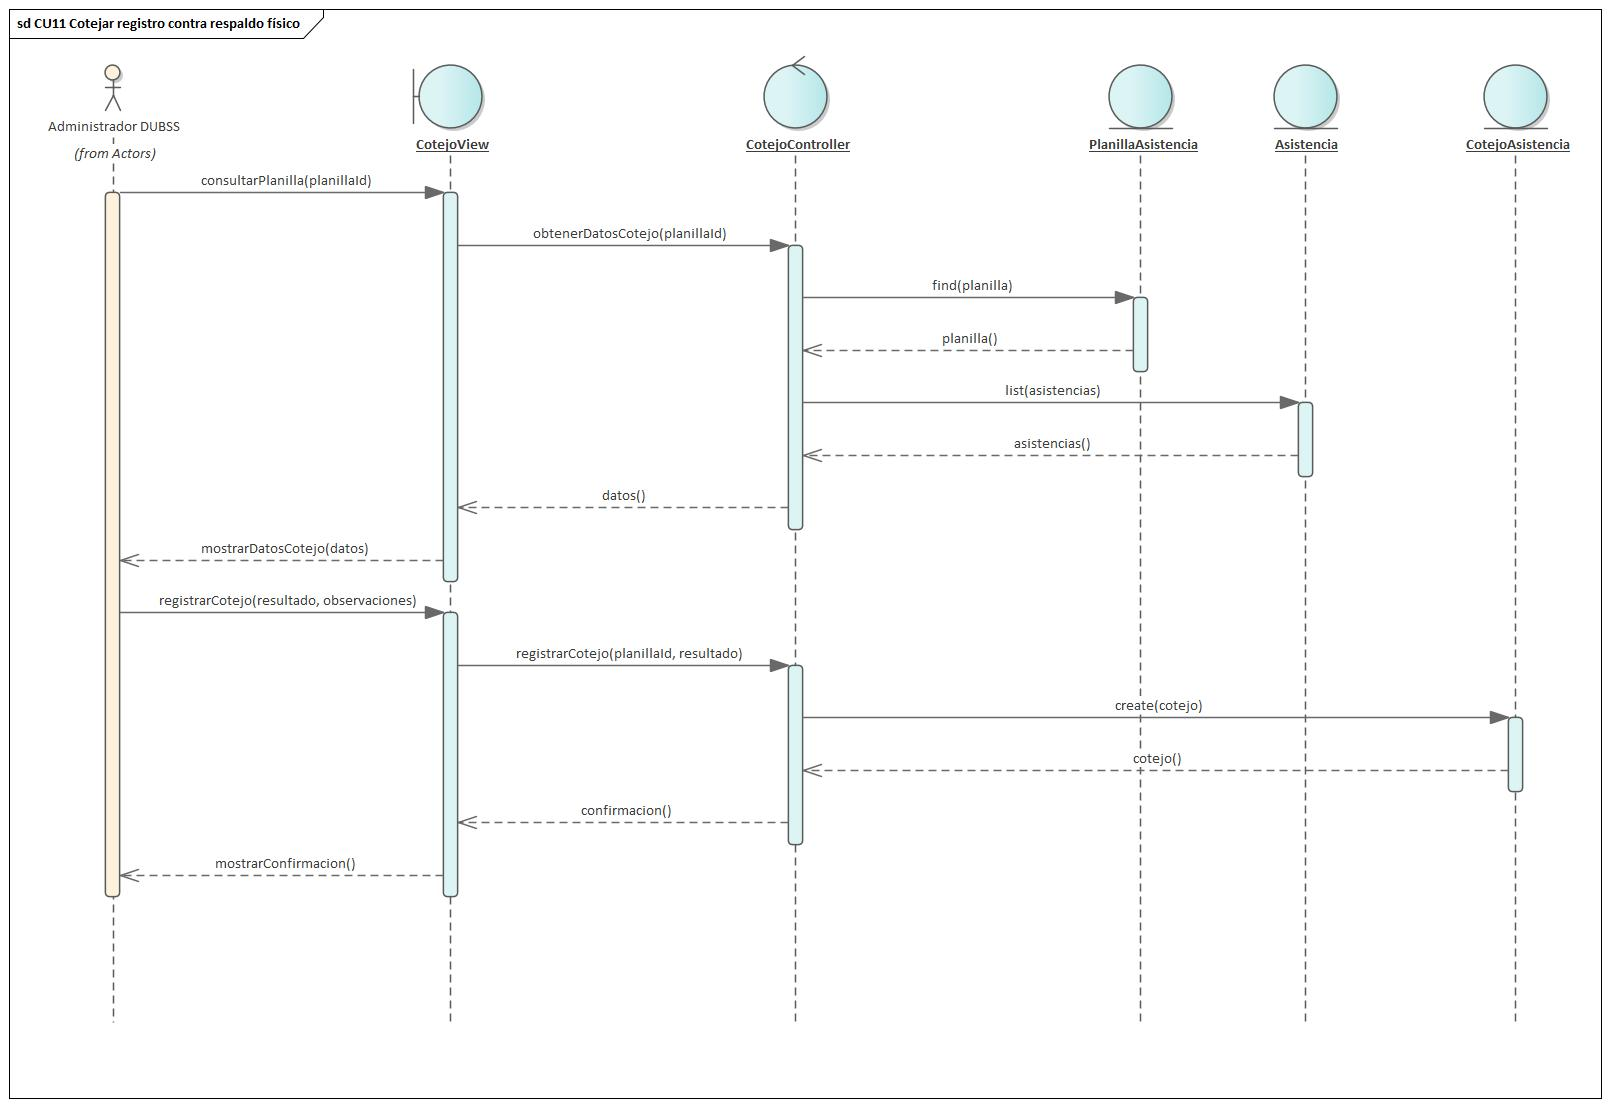
\includegraphics[width=\textwidth,height=0.75\textheight,keepaspectratio]{images/098_Secuencia_CU11_Cotejar_Registro_Respaldo_Fisico.jpg}

\smallskip
\noindent\raggedright\textit{Nota.} Elaboración propia.
\end{figure}


\subsubsection{7.4.12. Diseñar CU-12 Visualizar dashboard de indicadores BI}\label{sec:cap7_disenar_cu12}

La Figura~\ref{fig:secuencia_cu12} presenta el diagrama de secuencia del CU-12.

\begin{figure}[H]
\caption{Diagrama de secuencia del CU-12 Visualizar dashboard de indicadores BI}
\label{fig:secuencia_cu12}
\centering
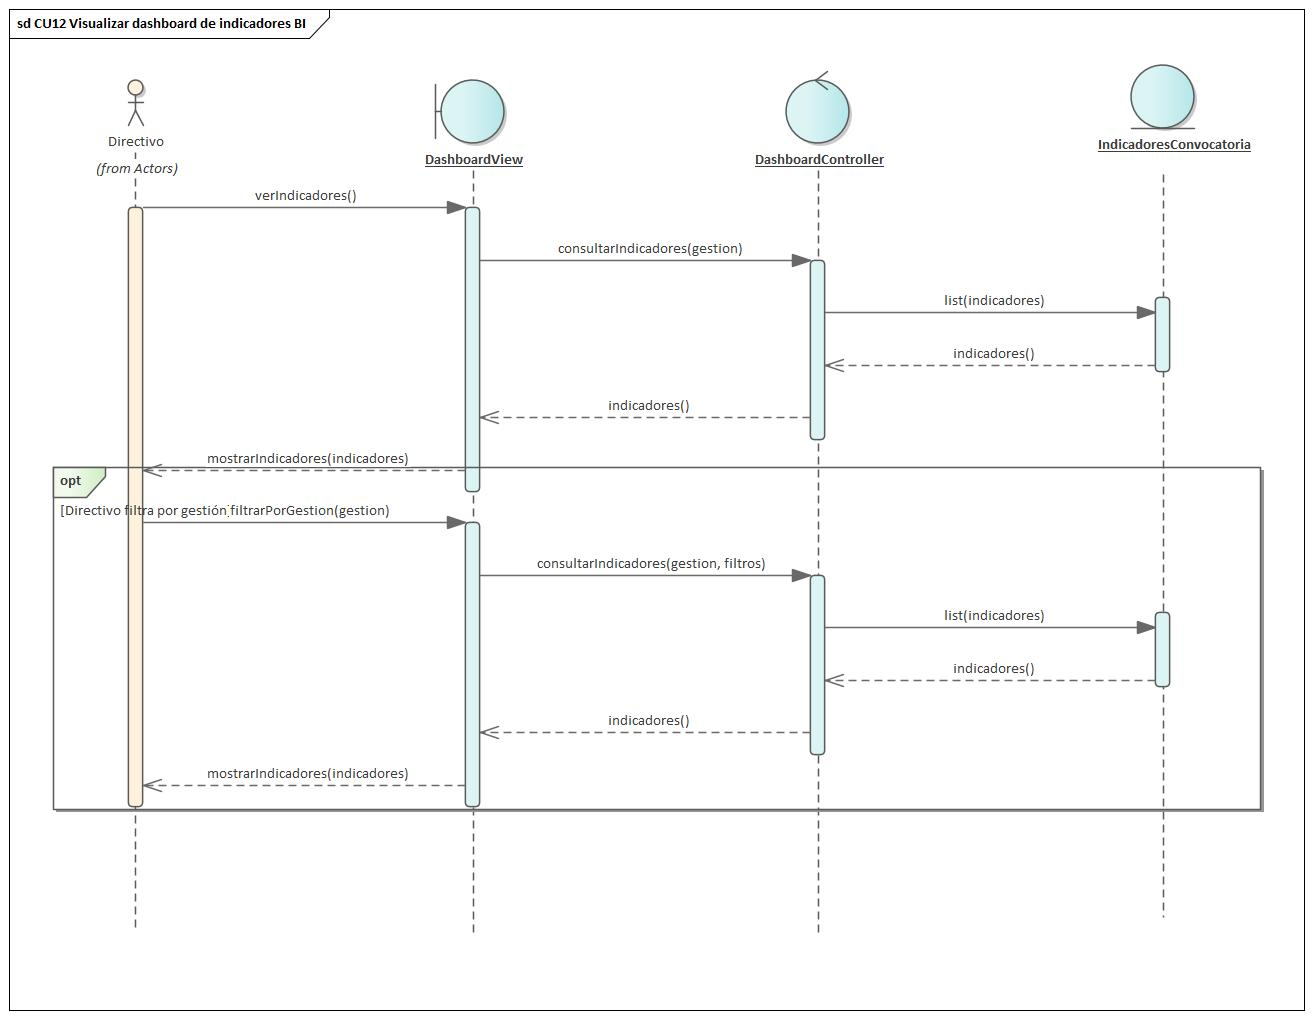
\includegraphics[width=\textwidth,height=0.75\textheight,keepaspectratio]{images/099_Secuencia_CU12_Visualizar_Dashboard_Indicadores_BI.jpg}

\smallskip
\noindent\raggedright\textit{Nota.} Elaboración propia.
\end{figure}


\subsubsection{7.4.13. Diseñar CU-13 Gestionar convocatoria y gestión académica}\label{sec:cap7_disenar_cu13}


\subsubsection{7.4.14. Diseñar CU-14 Gestionar usuarios y roles}\label{sec:cap7_disenar_cu14}


\subsubsection{7.4.15. Diseñar CU-15 Recuperar contraseña / gestionar perfil}\label{sec:cap7_disenar_cu15}


\subsubsection{7.4.16. Diseñar CU-16 Digitalizar y adjuntar documentos}\label{sec:cap7_disenar_cu16}


\subsubsection{7.4.17. Diseñar CU-17 Guardar borrador de postulación}\label{sec:cap7_disenar_cu17}


\subsubsection{7.4.18. Diseñar CU-18 Validar elegibilidad y duplicados}\label{sec:cap7_disenar_cu18}


\subsubsection{7.4.19. Diseñar CU-19 Devolver postulación para corrección}\label{sec:cap7_disenar_cu19}

La Figura~\ref{fig:secuencia_cu19} presenta el diagrama de secuencia del CU-19.

\begin{figure}[H]
\caption{Diagrama de secuencia del CU-19 Devolver postulación para corrección}
\label{fig:secuencia_cu19}
\centering
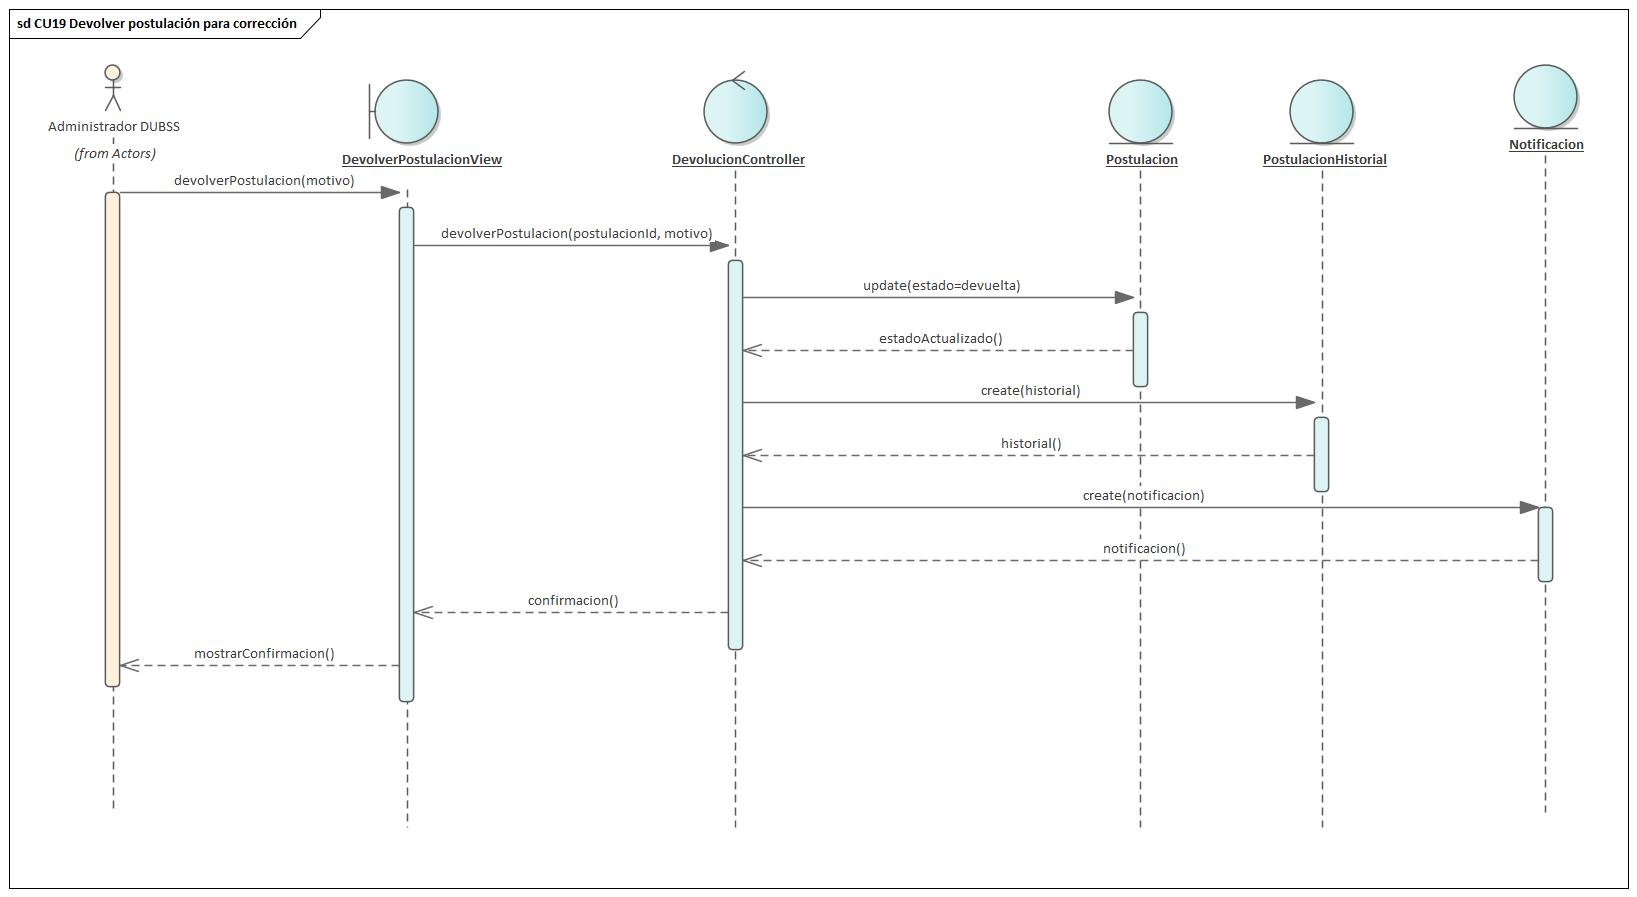
\includegraphics[width=\textwidth,height=0.75\textheight,keepaspectratio]{images/100_Secuencia_CU19_Devolver_Postulacion_Correccion.jpg}

\smallskip
\noindent\raggedright\textit{Nota.} Elaboración propia.
\end{figure}


\subsubsection{7.4.20. Diseñar CU-20 Archivar o rechazar postulación}\label{sec:cap7_disenar_cu20}

La Figura~\ref{fig:secuencia_cu20} presenta el diagrama de secuencia del CU-20.

\begin{figure}[H]
\caption{Diagrama de secuencia del CU-20 Archivar o rechazar postulación}
\label{fig:secuencia_cu20}
\centering
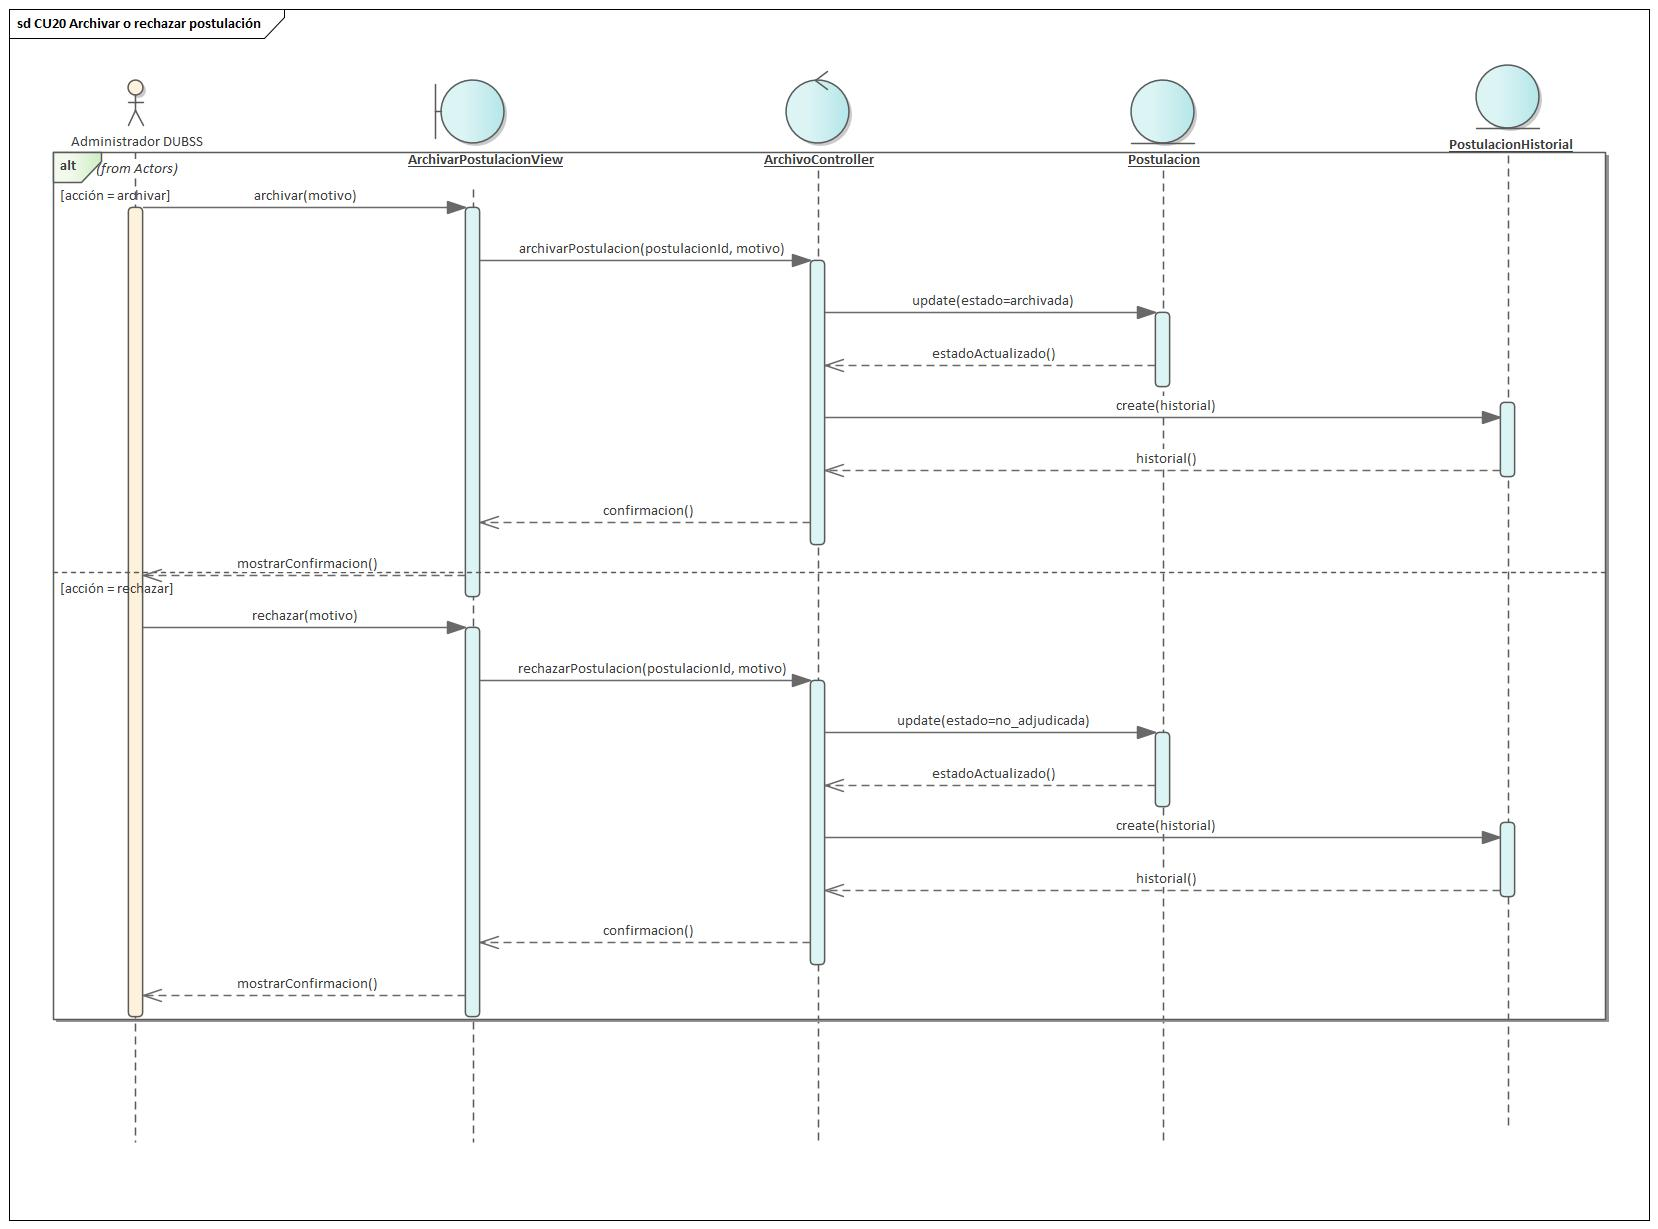
\includegraphics[width=\textwidth,height=0.75\textheight,keepaspectratio]{images/101_Secuencia_CU20_Archivar_Rechazar_Postulacion.jpg}

\smallskip
\noindent\raggedright\textit{Nota.} Elaboración propia.
\end{figure}


\subsubsection{7.4.21. Diseñar CU-21 Notificar finalistas, registrar entrega de documentación física y publicar comunicados/avisos}\label{sec:cap7_disenar_cu21}


\subsubsection{7.4.22. Diseñar CU-22 Publicar resultados de adjudicación}\label{sec:cap7_disenar_cu22}

La Figura~\ref{fig:secuencia_cu22} presenta el diagrama de secuencia del CU-22.

\begin{figure}[H]
\caption{Diagrama de secuencia del CU-22 Publicar resultados de adjudicación}
\label{fig:secuencia_cu22}
\centering
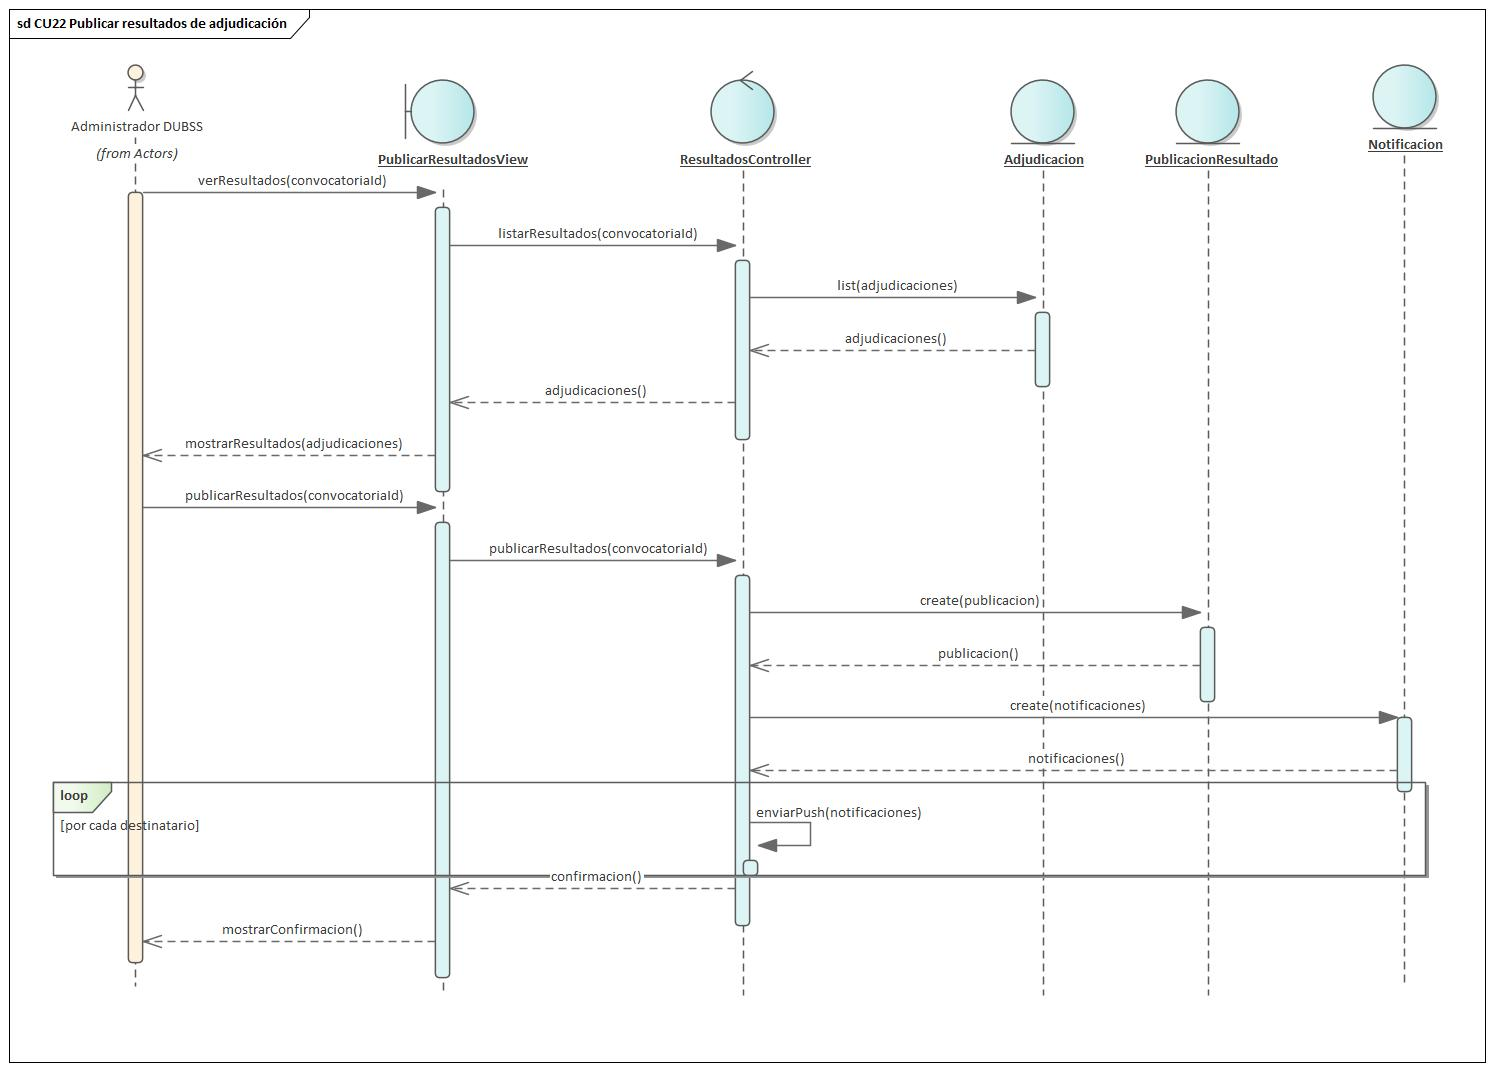
\includegraphics[width=\textwidth,height=0.75\textheight,keepaspectratio]{images/102_Secuencia_CU22_Publicar_Resultados_Adjudicacion.jpg}

\smallskip
\noindent\raggedright\textit{Nota.} Elaboración propia.
\end{figure}


\subsubsection{7.4.23. Diseñar CU-23 Gestionar padrón de becados (baja, suspensión, reemplazo)}\label{sec:cap7_disenar_cu23}

La Figura~\ref{fig:secuencia_cu23} presenta el diagrama de secuencia del CU-23.

\begin{figure}[H]
\caption{Diagrama de secuencia del CU-23 Gestionar padrón de becados (baja, suspensión, reemplazo)}
\label{fig:secuencia_cu23}
\centering
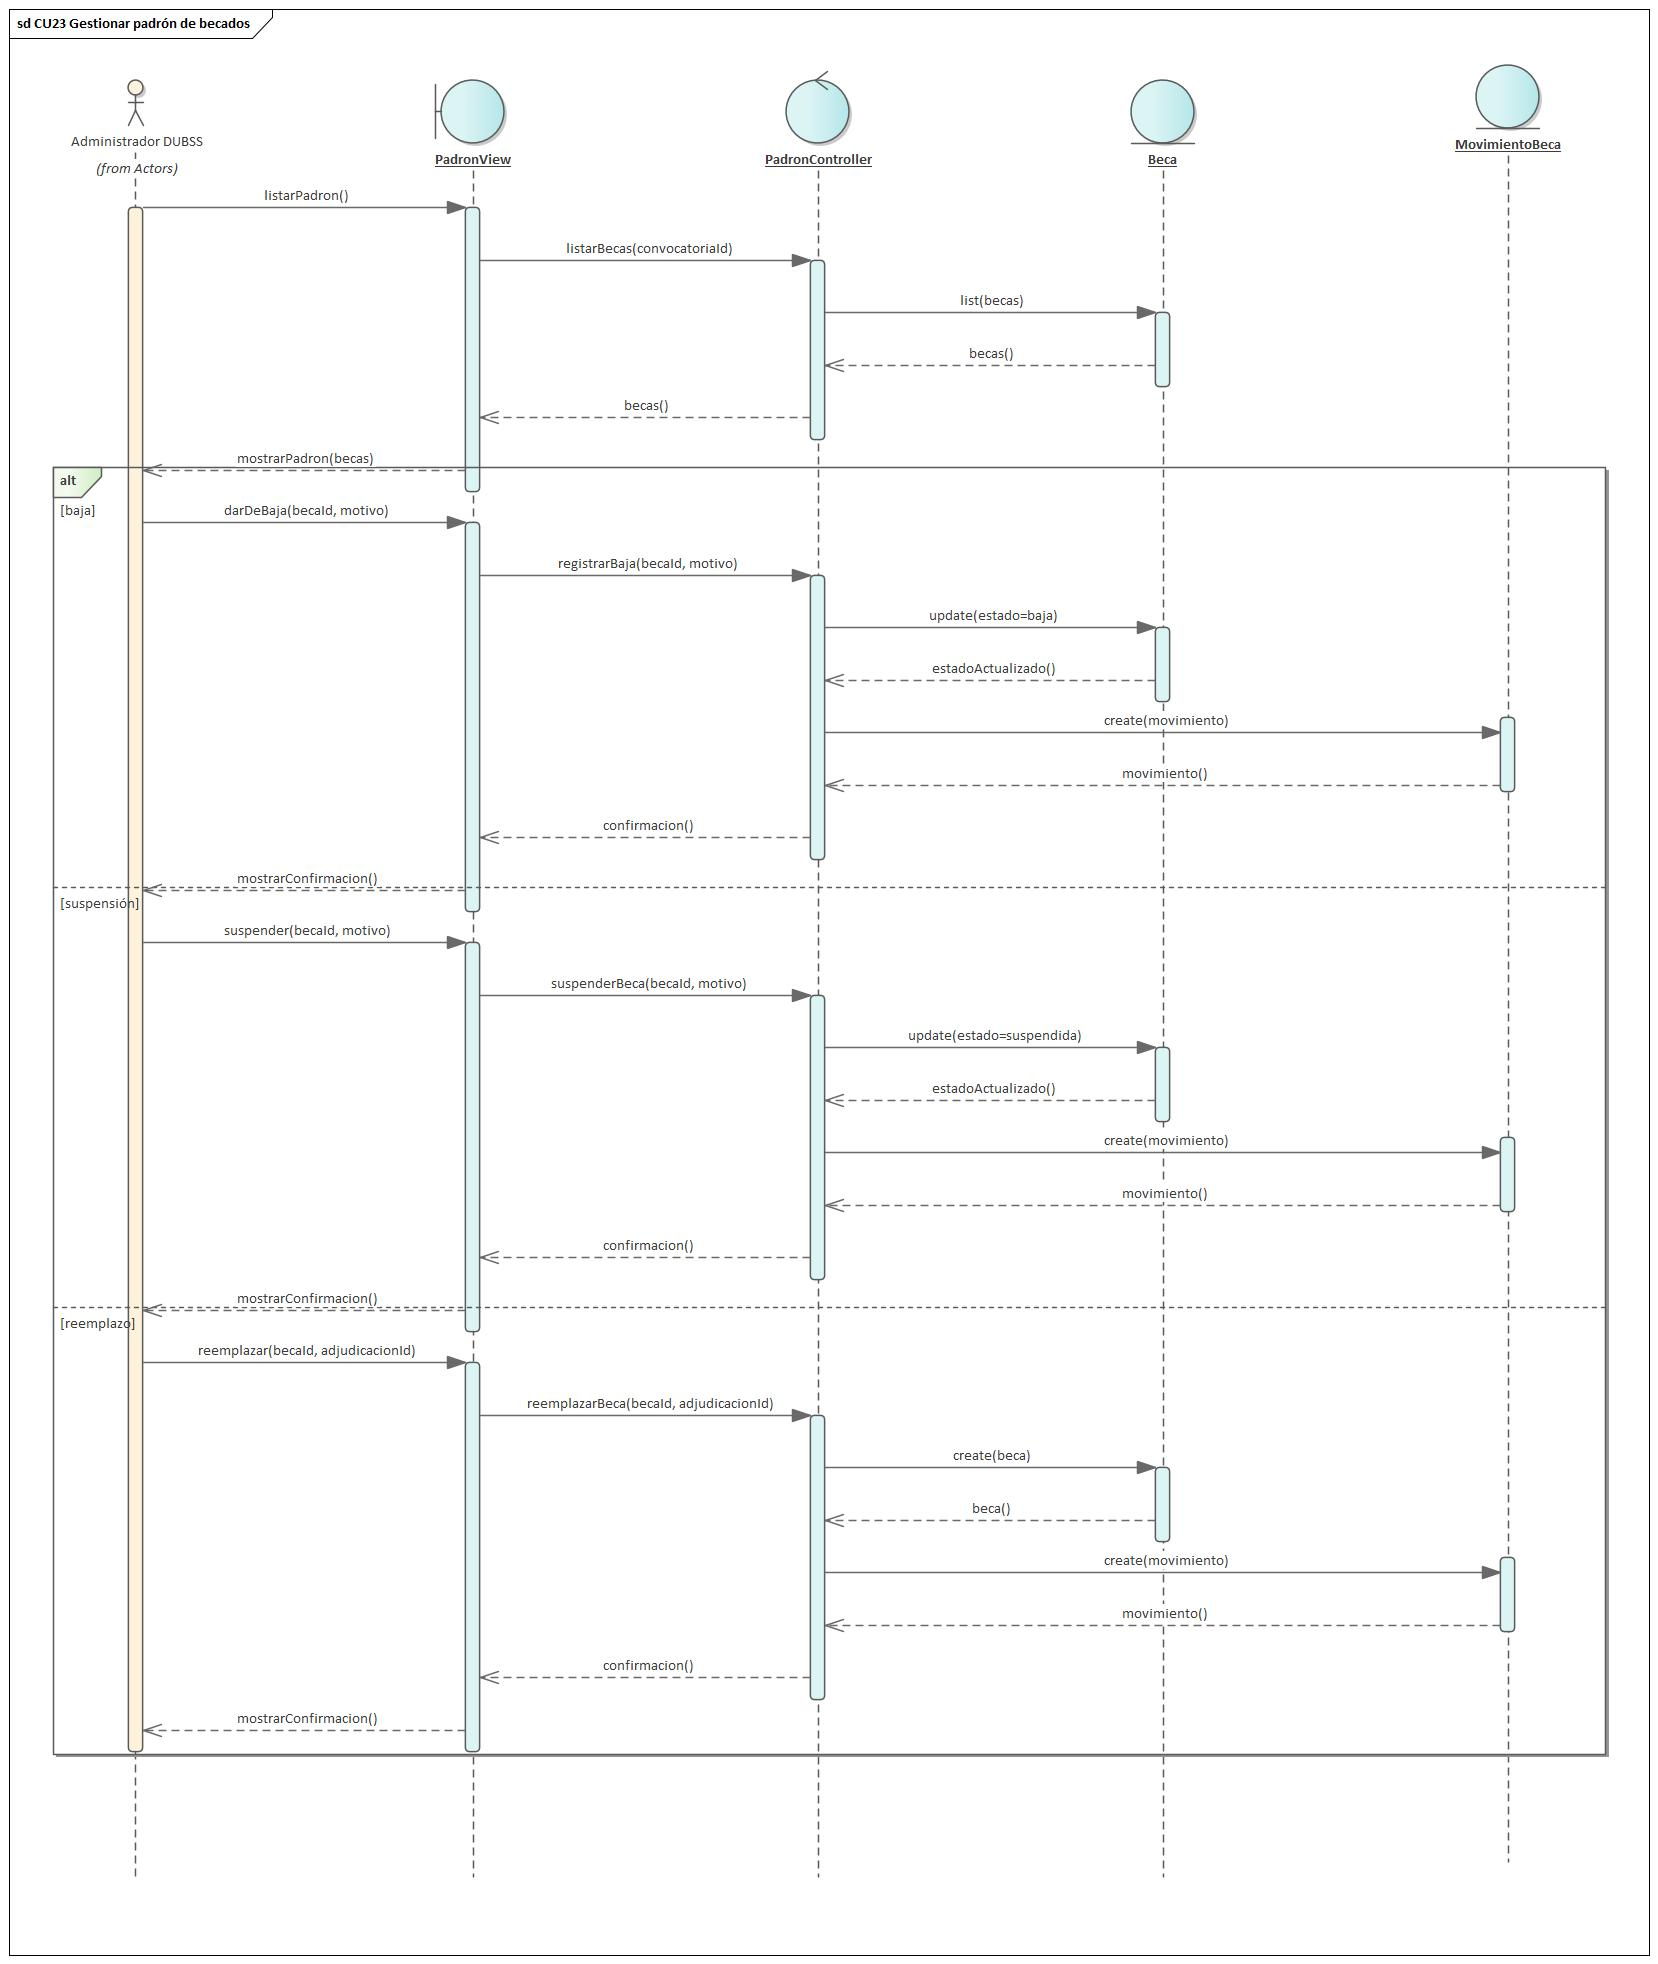
\includegraphics[width=\textwidth,height=0.75\textheight,keepaspectratio]{images/103_Secuencia_CU23_Gestionar_Padron_Becados.jpg}

\smallskip
\noindent\raggedright\textit{Nota.} Elaboración propia.
\end{figure}


\subsubsection{7.4.24. Diseñar CU-24 Consultar historial de asistencia y estado de beca}\label{sec:cap7_disenar_cu24}


\subsubsection{7.4.25. Diseñar CU-25 Consultar bitácora de acciones}\label{sec:cap7_disenar_cu25}

La Figura~\ref{fig:secuencia_cu25} presenta el diagrama de secuencia del CU-25.

\begin{figure}[H]
\caption{Diagrama de secuencia del CU-25 Consultar bitácora de acciones}
\label{fig:secuencia_cu25}
\centering
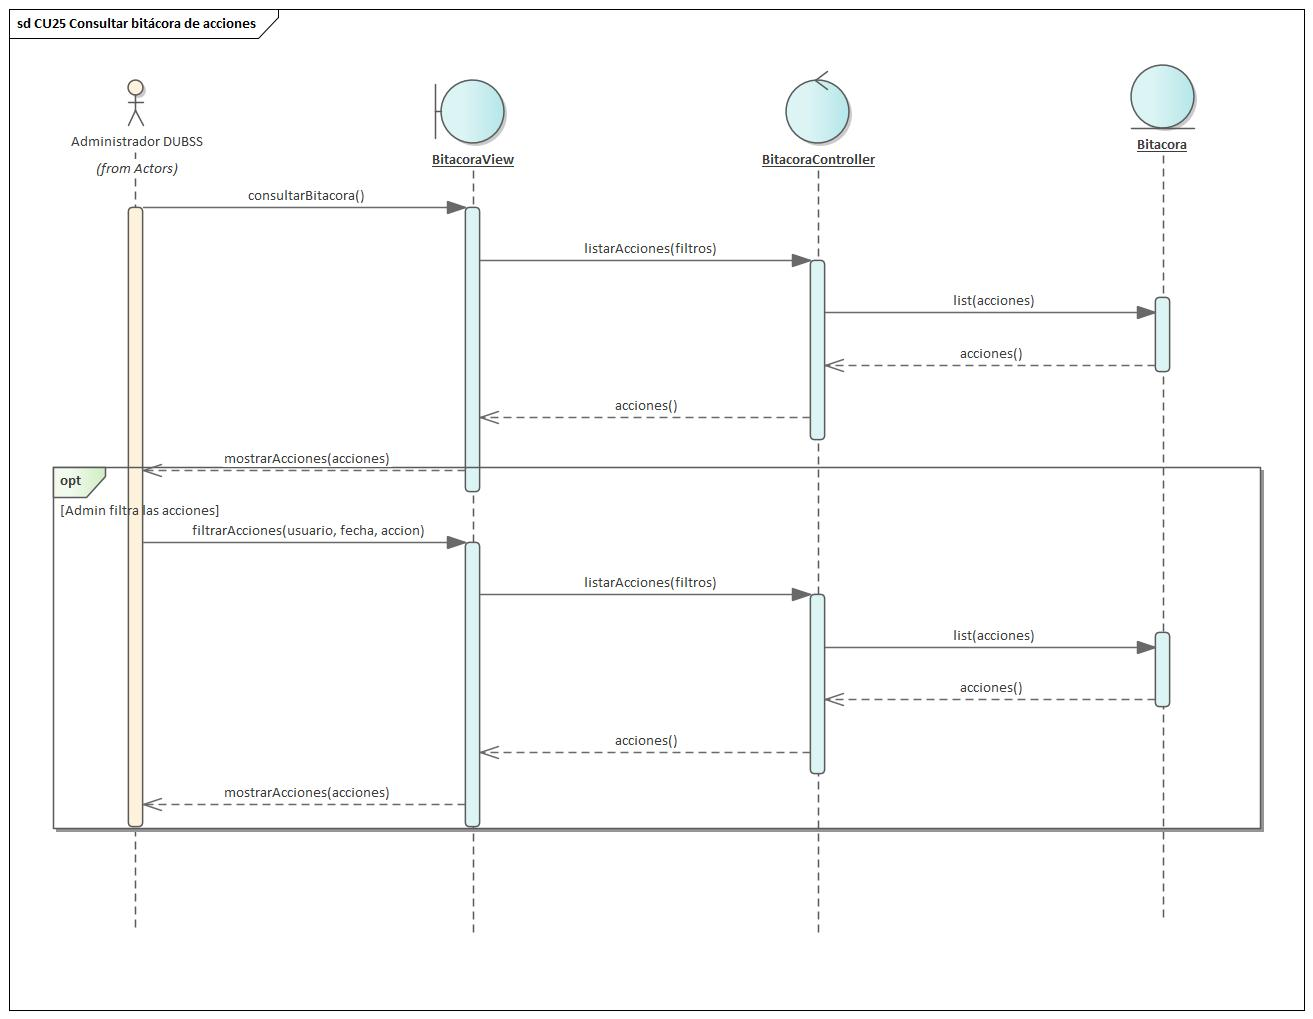
\includegraphics[width=\textwidth,height=0.75\textheight,keepaspectratio]{images/104_Secuencia_CU25_Consultar_Bitacora_Acciones.jpg}

\smallskip
\noindent\raggedright\textit{Nota.} Elaboración propia.
\end{figure}


\subsubsection{7.4.26. Diseñar CU-26 Parametrizar modelo de preselección y reprocesar puntajes}\label{sec:cap7_disenar_cu26}

